\documentclass{article}
\usepackage{graphicx} % Required for inserting images
\usepackage[top=0.9in, bottom=1in, left=1.5in, right=1.5in]{geometry}
\usepackage[utf8]{inputenc}
\usepackage[icelandic]{babel}
\usepackage[T1]{fontenc}
\usepackage[sc]{mathpazo}
\usepackage[parfill]{parskip}
\renewcommand{\baselinestretch}{1.2}
\usepackage{booktabs,tabularx}
\usepackage{multirow}
\usepackage{enumerate}
\usepackage{adjustbox}
\usepackage{multicol}
\usepackage{xcolor}
\usepackage{algpseudocode}
\usepackage{tikz}
\usepackage{nicefrac}
\usepackage{changepage}
\usetikzlibrary{arrows, positioning, calc, graphs}
\usepackage{amsmath, amsfonts, amssymb, amsthm}
\usepackage{graphicx}
\usepackage{tikz}
\usepackage{minted}
\usemintedstyle{manni}
\title{Tölvutækni og Forritun Heimadæmi 8 }
\author{Ragnar Björn Ingvarsson, rbi3}
\tikzset{->, >=stealth', shorten >=1pt, node distance=2cm,thick, main node/.style={circle,draw,minimum size=3em}}

\begin{document}
\renewcommand\thepage{}

	\maketitle

	\newpage
	\setcounter{page}{1}
	\renewcommand\thepage{\arabic{page}}

	\section{}
	Við tökum eftir skv. vísbendingu að \textbf{A} hefur \textbf{N } dálka 
	og \textbf{B} hefur \textbf{M} dálka. Þá notum við formúlu sem sýnd 
	var í fyrirlestri, 
	\begin{equation}
		\text{Vistfang: } A + i \cdot (C \cdot K) + j \cdot K
		\label{eq:Aðgangur í 16x16 fylki}
	\end{equation}
	Og sjáum að þar sem margfaldað er í smalamálskóðanum með $K$ í lokin, 
	er formúlan
	\begin{equation}
		\text{Vistfang: } A + i \cdot C + j
		\label{eq:adjusted}
	\end{equation}
	Þá vitum við að þar sem $\%rdi$ er margfaldað með $6$ í kóðanum hlýtur 
	$C = 6$ fyrir $A$, en þar sem $\%rsi$ er margfaldað með $10$ er $C = 10$ 
	fyrir $B$. Þar af leiðandi er $N = 6$ og $M = 10$. Þetta fæst frá 
	því að vita að til að fá rétta dálkinn í $A$ og $B$ þarf að hoppa í 
	gegn um $i$ margar raðir. Hver röð er þá af stærð fjölda dálka svo við 
	vitum að ef þarf að hafa $6i$ til að komast í gegn um allar raðirnar 
	hlýtur fjölda dálka að vera fastinn $6$. Og sama gengur með $B$.

	\section{}
	\begin{itemize}
		\item[a)] Við sjáum að fyrst upphafsvistfangið er $100$ fáum við 
			jöfnuna
			\begin{equation}
				100 + i\cdot (C\cdot K) + j\cdot K
				\label{eq:gamer}
			\end{equation}

			Þar sem $i = 3$, $j = 4$, $C = 10$ og $K = 2$ þar sem 
			\textit{short int }í c er 16 bitar eða $2$ bæti. Við vitum 
			einnig að $C = 10$ þar sem $C$ er fjöldi dálka og táknar í raun 
			stærð hverrar raðar. Skv. þessu fæst
			\begin{equation}
				100 + 3\cdot 10\cdot 2 + 4\cdot 2= 100 + 60 + 8 = 168
				\label{eq:gamer1}
			\end{equation}
		\item[b)] Í heild sinni tekur færslan $32$ bæti:

			\begin{center}
				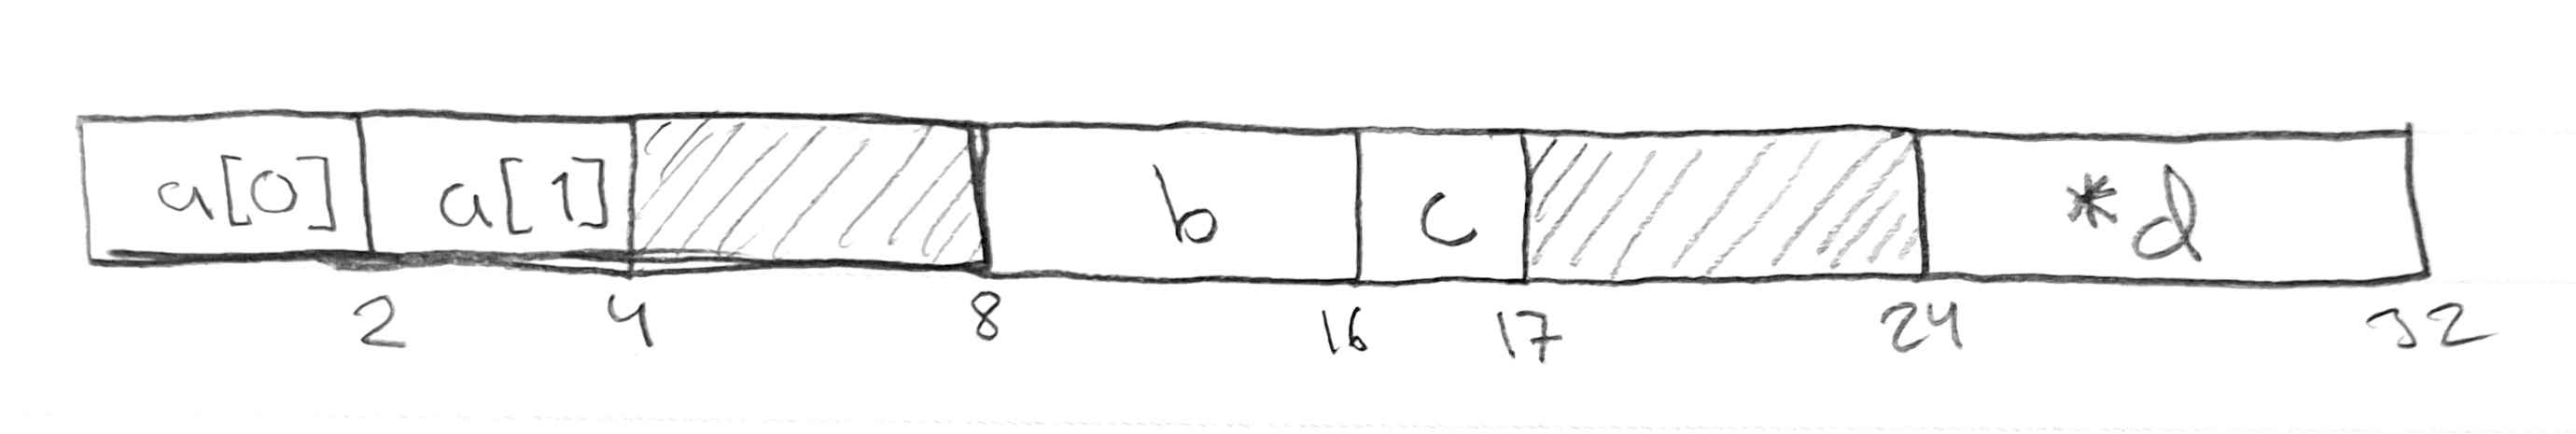
\includegraphics[scale=0.11]{gmaer.jpg}
			\end{center}
	\end{itemize}
	
	\section{}

	Ef við þýðum foritið með \textbf{-Og} og \textbf{-fstack-protector} þá 
	fæst að kanarígildið byrjar sem $0$ en með hverjum auka staf sem 
	skrifaður er í inntakið hækkar $\%rax$ um einn, þ.m.t. newline character.

	Svo kanarífuglagildið $\%rax$ er alltaf jafnt lengd inntaksstrengsins 
	plús einn.

	\section{}
	\begin{itemize}
		\item[a)] Í fyrsta lagi er $\%rcx$ notað í stað þess að framkvæma 
			alla reikningana inni í lykkjunni, það virkar svo að þar sem 
			við vitum að $A$ er fylki af stærð \textit{long} þá getum við 
			sagt að í hverri ítrun viljum við bæta við $8(n+1)$ í 
			fylkisaðganginn okkar svo $\%rcx$ virkar sem þetta gildi. 
			Síðan er $\%rax$ notað sem teljari og við bætum einum við hann 
			í hverri ítrun og athugum svo hvort hann sé jafn $\%rsi$. 
			Síðan er $\%rdx$, eða $val$ einfaldlega bætt við núverandi 
			stak í fylkisaðganginum okkar í hverri ítrun.
		\item[b)] Tilgangur þessarrar skipanar er að besta burt þörfina á 
			því að reikna $i\cdot n + 1$ í hverri ítrun fallsins og í 
			stað þess er hægt að plúsa bara við $n+1$ í hverri ítrun þar 
			sem við vitum að $i$ hækkar alltaf bara um $1$. Einnig er allt 
			margfaldað með $8$ þar sem við erum að vinna með fylki af tagi 
			\textit{long}.
		\item[c)] Það er óþarfi að vinna með margföldun vegna þess að 
			fylkisaðgangurinn er hækkaður línulega með hverri ítrun svo 
			hægt er að taka þessa hækkun út fyrir lykkjuna og plúsa svo 
			einfaldlega við í hverri ítrun.
	\end{itemize}

	\section{}
	\begin{itemize}
		\item[a)] Við sjáum að í báðum tilfellum er verið að nota minni 
			fyrir summuna, tökum eftir skipununum 

			\texttt{ 1167:	48 01 0a             	add    \%rcx,(\%rdx)} og 

			\texttt{ 1157:	48 89 02             	mov    \%rax,(\%rdx)}

			þar sem í báðum tilfellum er verið að gera skipunina inni í lykkjunni.

		\item[b)] Getum einfaldlega bætt við breytu \texttt{sum} og plúsað 
			alltaf við hana og svo fært lokagildið inn í \texttt{*res}. 

			\begin{minted}{c}
void fun(long *a, int len, long *res) {
    int i;
    int sum = 0;
  
    for (i=0; i<len; i++)
        sum += a[i];
    *res = sum;
}
			\end{minted}
	\end{itemize}

	Sem endar í smalamálskóðanum 

	\begin{verbatim}
0000000000001140 <fun>:
    1140:	48 c7 02 00 00 00 00 	movq   $0x0,(%rdx)
    1147:	b9 00 00 00 00       	mov    $0x0,%ecx
    114c:	b8 00 00 00 00       	mov    $0x0,%eax
    1151:	eb 17                	jmp    116a <fun+0x2a>
    1153:	66 66 2e 0f 1f 84 00 	data16 cs nopw 0x0(%rax,%rax,1)
    115a:	00 00 00 00 
    115e:	66 90                	xchg   %ax,%ax
    1160:	4c 63 c0             	movslq %eax,%r8
    1163:	42 03 0c c7          	add    (%rdi,%r8,8),%ecx
    1167:	83 c0 01             	add    $0x1,%eax
    116a:	39 f0                	cmp    %esi,%eax
    116c:	7c f2                	jl     1160 <fun+0x20>
    116e:	48 63 c9             	movslq %ecx,%rcx
    1171:	48 89 0a             	mov    %rcx,(%rdx)
    1174:	c3                   	ret
	\end{verbatim}

	Þar sem vert er að athuga að inni í lykkjunni frá 1160 til 116a er ekki 
	verið að færa gildið frá $a$ inn í minni heldur er því bætt við $\%ecx$ 
	og svo er $\%ecx$ fært inn í $(\%rdx)$ í lokin.

	\section{}

	Við sjáum hér um leið að verið er að lesa inntakið okkar inn í minni 
	sem byrjar þá á $\%rsp$, svo er verið að sleppa fyrstu $8$ bætunum og 
	bera það svo við gildið $0x3930334c96c354$. Með því að athuga á minninu 
	sem prentað er frá á mismunandi stöðunum þar sem kallað er á \texttt{puts} 
	er hægt að sjá að við viljum fá að inntaksstrengurinn okkar, fyrir utan 
	fyrstu $8$ bætin á að vera jafn stóru hex tölunni.

	Með því að prófa smá sést að bætin eru borin saman við töluna í öfugri 
	röð svo fyrst þarf að koma $54$, svo $c3$ o.s.frv.

	Við athugum bara á ascii töflu og sjáum að $54$ er T, $c3$ er ekki til 
	eitt og sér svo við sjáum að það eru til útgáfur af þvi sem eru tvö bæti 
	og heppilega er til $c3$ $96$ sem er Ö, svo kemur $4c$ sem er L og 
	síðan kemur $3$, $0$ og loks $9$. 

	Þaðan af sést að fyrir utan fyrstu $8$ stafina þarf strengurinn að vera 
	TÖL309, svo við prófum aaaaaaaaTÖL309 sem virkar!
	
\end{document}
